\documentclass[11pt,a4paper]{article}
\usepackage[T1]{fontenc}
\usepackage{isabelle,isabellesym}
\usepackage{graphicx}
\usepackage{amssymb}
\usepackage{euromils}

\docnumber{D31.1}
\doctitle{Formal Specification of a Generic Separation Kernel}

\doctype{R}

\docactivity{Activity~3}
\docwp{WP~3.1}

% due date
\docdate{
    \formatdate{30}{09}{2013} % {DD}{MM}{YYYY} 
}
\docmonth{12}

% responsible organisation
\organisation{Open University of The Netherlands}

% editor
\doceditor{Freek Verbeek, Julien Schmaltz}

% authors
\docauthor{%
Sergey Tverdyshev, Oto Havle, Holger Blasum (SYSGO AG)\\
Bruno Langenstein, Werner Stephan (Deutsches Forschungszentrum f\"{u}r k\"{u}nstliche Intelligenz / DFKI GmbH)\\
Abderrahmane Feliachi, Yakoub Nemouchi, Burkhart Wolff (Universit\'{e} Paris Sud)\\
Freek Verbeek, Julien Schmaltz (Open University of The Netherlands)} 

\doctag{PU}

% revision
\docversion{0.0}
\docrevision{\svnrev}

% abstract and keywords
\docabstract{
We introduce a theory of intransitive non-interference for separation kernels 
with control. We show that it can be instantiated for a simple API consisting 
of IPC and events.}
\dockeywords{separation kernel with control, formal model, instantiation, IPC, events, Isabelle/HOL}

\executivesummary{
%We introduce a theory of intransitive non-interference for separation kernels with %control. We show that it can be instantiated for a simple API consisting of IPC and %events.
%}
%
%\abstract{
Intransitive noninterference has been a widely studied topic in the last few 
decades. Several well-established methodologies apply interactive theorem 
proving to formulate a noninterference theorem over abstract academic models. 
In joint work with several industrial and academic partners throughout Europe,
we are helping in the certification process of PikeOS, an industrial separation 
kernel developed at SYSGO. In this process, established theories could not be 
applied. We present a new generic model of separation kernels and a new theory 
of intransitive noninterference. The model is rich in detail, making it suitable 
for formal verification of realistic and industrial systems such as PikeOS. 
Using a refinement-based theorem proving approach, we ensure that proofs remain 
manageable.

This document corresponds to the deliverable D31.1 of the EURO-MILS Project
\url{http://www.euromils.eu}.
}

\usepackage{MnSymbol}

% this should be the last package used
\usepackage{pdfsetup}

% urls in roman style, theory text in math-similar italics
\urlstyle{rm}
\isabellestyle{it}

\begin{document}

\euromilsmaketitlelists
\clearpage

\section{Introduction}
%CONTEXT: separation kernels, verification of PikeOS, intransitive noninterference\\
Separation kernels are at the heart of many modern security-critical systems~\cite{rushby81}.
With next generation technology in cars, aircrafts and medical devices becoming 
more and more interconnected, a platform that offers secure decomposition of 
embedded systems becomes crucial for safe and secure performance.
PikeOS, a separation kernel developed at SYSGO, is an operating system providing 
such an environment~\cite{kaiser07,brygier09}.
A consortium of several European partners from industry and academia works on 
the certification of PikeOS up to at least Common Criteria EAL5+, with "+" 
being applying formal methods compliant to EAL7.
Our aim is to derive a precise model of PikeOS and a precise formulation of the 
PikeOS security policy.%, to be used for the Common Criteria evaluation of PikeOS.

A crucial security property of separation kernels is \emph{intransitive} \emph{noninterference}.
This property is typically required for systems with multiple independent levels 
of security (MILS) such as PikeOS. It ensures that a given security policy over 
different subjects of the system is obeyed. Such a security policy dictates 
which subjects may flow information to which other subjects.


%MOTIVATION: Certification of PikeOS: Rushby/GWV/etc. not usable for realistic, industrial systems.
Intransitive noninterference has been an active research field for the last 
three decades. Several papers have been published on defining intransitive 
noninterference and on unwinding methodologies that enable the proof of 
intransitive noninterference from local proof obligations. However, in the 
certification process of PikeOS these existing methodologies could not be directly 
applied. Generally, the methodologies are based on highly abstract generic 
models of computation. The gap between such an abstract model and the reality of 
PikeOS is large, making application of the methodologies tedious and cumbersome.

%CONTRIBUTION: new model + new theory
This paper presents a new generic model for separation kernels called CISK 
(for: Controlled Interruptible Separation Kernel). This model is richer in 
details and contains several facets present in many separation kernels, such as 
\emph{interrupts}, \emph{context} \emph{switches} between domains and a notion of 
\emph{control}. Regarding the latter, this concerns the fact that the kernel 
exercises control over the executions as performed by the domains.
The kernel can, e.g., decide to skip actions of the domains, or abort them halfway.
We prove that any instantiation of the model provides intransitive noninterference.
The model and proofs have been formalized in Isabelle/HOL~\cite{nipkow12} 
which are included in the subsequent sections of this document.
%\footnote{Source code is available at: removed for double blind review.}.
%DOUBLEBLIND\\\url{www.cs.ru.nl/~freekver/EUROMILS/CSF14.zip}}.


We have adopted Rushby's definition of intransitive noninterference~\cite{rushby92}.
We first present an overview of our approach and then discuss the relation between 
our approach and existing methodologies in the next section.
%Our definition improves on Rushby's ipurge-based (for: intransitive purge)  definition in two ways.
%First, we do not assume a static mapping of actions to domains, since for an OS kernel such a mapping does not necessarily exist~\cite{murray12}.
%Secondly, we prove more directly that domains perform securely in presence of attackers.
%Instead of removing actions, we replace the program code of an attacking domain by arbitrary other program code from the attack surface.

% PAPER OVERVIEW
%We first present the generic model and the security theorem that is proven for it in Section~\ref{sec:theorem}.
%We then present our locale-based approach in Section~\ref{sec:proofs}.
%Related work is presented in Section~\ref{sec:related}.
%We conclude in Section~\ref{sec:conclusion}.

\subsubsection*{Overview}\label{subsec:overview}

Generally, there are two conflicting interests when using a generic model.
On the one hand the model must be sufficiently abstract to ensure that theorems 
and proofs remain manageable. On the other hand, the model must be rich enough 
and must contain sufficient domain-knowledge to allow easy instantiation.
Rushby's model, for example, is on one end of the spectrum: it is basically a 
Mealy machine, which is a highly abstract notion of computation, consisting only 
of state, inputs and outputs~\cite{rushby92}.
The model and its proofs are manageable, but making a realistic instantiation is 
tedious and requires complicated proofs. %and quickly becomes infeasible.

We aim at the other side of the spectrum by having a generic model that is rich in detail.
As a result, instantiating the model with, e.g., a model of PikeOS can be done easily.
To ensure maintainability of the theorems and proofs, we have applied a highly 
modularized theorem proving technique.
% based on Isabelles' \emph{locales}.
%Locales basically allowed us a separation of concerns, i.e., they allowed us to separate different facets of the model.

%Starting with a highly generic and abstract model of a separation kernel, we define and prove security for this model.
%Then, the model is enriched step-by-step.
%As each step is an extension of the previous step, all the proofs can be automatically reused.
%This methodology ensures manageable proofs.
%The result of these locale-based proofs is a rich generic model that can be instantiated easily.

Figure~\ref{fig:extensions} shows an overview.
The initial module ``Kernel'' is close to a Mealy machine, but has several 
facets added, including interrupts, context switches and control.
New modules are added in such a way that each new module basically inserts an 
adjective before ``Kernel''.
The use of modules allows us to prove, e.g., a separation theorem in module 
``Separation Kernel'' and subsequently to reuse this theorem later on when details 
on control or interrupts are added.
\begin{figure}[htb]
\centering
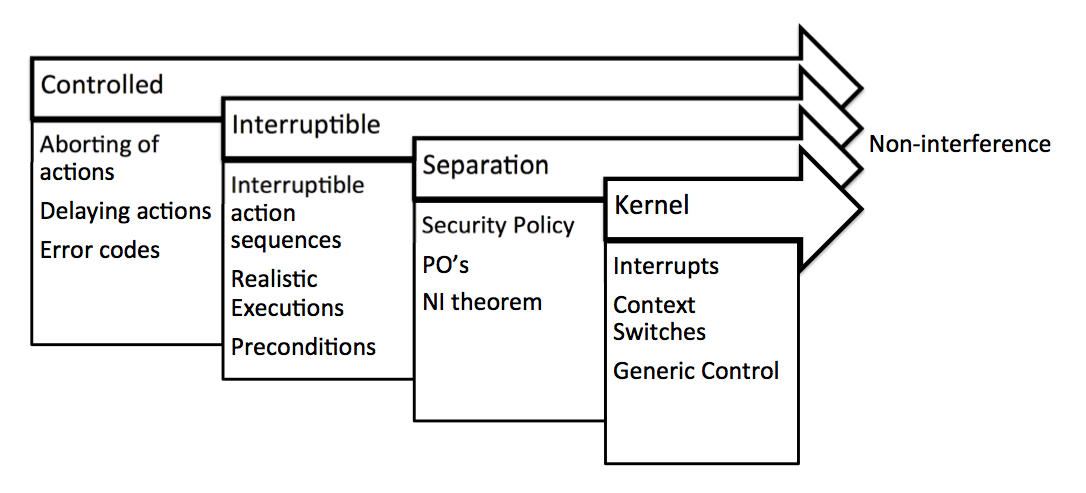
\includegraphics[width=\linewidth]{locales.png}
\caption{Overview of CISK modular structure}
\label{fig:extensions}
\end{figure}
% TODO


The second module adds a notion of separation, yielding a module of a Separation 
Kernel (SK). A security policy is added that dictates which domains may flow 
information to each other. Local proof obligations are added from which a global 
theorem of noninterference is proven. This global theorem is the \emph{unwinding} 
of the local proof obligations.
%The addition of a control mechanism to the model means that the traditional 
%formulation of intransitive noninterference no longer applies, as will be 
%explained in Section~\ref{sec:related}.
%We have reformulated noninterference to deal with control.

In the third module calls to the kernel are no longer considered atomic, 
yielding an Interruptible Separation Kernel (ISK).
In this model, one call to the kernel is represented by an \emph{action sequence}.
Consider, for example, an IPC call (for: Inter Process Communication). From the 
point of view of the programmer this is one kernel call. From the point of view 
of the kernel it is an action sequence consisting of three stages 
IPC\_PREP, IPC\_WAIT, and IPC\_SEND. 
During the PREP stage, it is checked whether the IPC is allowed by the security 
policy.
The WAIT stage is entered if a thread needs to wait for its communication partner.
The SEND stage is data transmission.
After each stage, an interrupt may occur that switches the current context.
A consequence of allowing interruptible action sequences is that it is no longer 
the case that any execution, i.e., any combination of atomic kernel actions, is 
realistic. We formulate a definition of \emph{realistic execution} and weaken 
the proof obligations of the model to apply only to realistic executions.

The final module provides an interpretation of control that allows atomic kernel 
actions to be aborted or delayed.
Additional proof obligations are required to ensure that noninterference is still 
provided.
This yields a Controlled Interruptible Separation Kernel (CISK).
When sequences of kernel actions are aborted, error codes can be transmitted to 
other domains.
Revisiting our IPC example, after the PREP stage the kernel can decide to abort 
the action. The IPC action sequence will not be continued and error codes may be 
sent out.
At the WAIT stage, the kernel can delay the action sequence until the communication 
partner of the IPC call is ready to receive.



% OLD
In Section~\ref{sect:generic} we introduce a theory of intransitive 
non-interference for separation kernels with control, based on~\cite{Verbeek2013}. 
We show that it can be instantiated for a simple API consisting of IPC and 
events (Section~\ref{sect:instantiation}). The rest of {\em this} section gives 
some auxiliary theories used for Section~\ref{sect:generic}.

\section{Preliminaries}

% generated text of all theories
\input{session}

\section{Related Work}
We consider various definitions of intransitive (I) nonin- terference (NI). 
This overview is by no means intended to be complete. We first prune the field 
by focusing on INI with as granularity the domains: if the security policy states 
the act ``$v \rightsquigarrow u$'', this means domain v is permitted to flow any information it has 
at its disposal to u. We do not consider language-based approaches to noninterference
\cite{SKIPaper6}, which allow finer granularity mechanisms (i.e., flowing just a subset of 
the available information). Secondly, several formal verification efforts have 
been conducted concerning properties similar and related to INI such as 
no-exfiltration and no-infiltration \cite{SKIPaper7}. Heitmeyer et al. prove these properties 
for a separation kernel in a Common Criteria certification process \cite{Heitmeyer:2006:FSV:1180405.1180448} 
(which kernel and which EAL is not clear). Martin et al. proved separation 
properties over the MASK kernel \cite{Martin:2000:FCM:786768.786973} and Shapiro and Weber verified correctness 
of the EROS confinement mechanism \cite{Shapiro:2000:VEC:882494.884422}. Klein provides an excellent overview of 
OS's for which such properties have been verified \cite{SKIPaper11}. Thirdly, INI definitions 
can be built upon either state-based automata, trace-based models, or process 
algebraic models \cite{SKIPaper12}. We do not focus on the latter, as our approach is not 
based on process algebra.

Transitive NI was first introduced by Goguen and Meseguer in 1982 \cite{SKIPaper13} and has 
been the topic of heavy research since. Goguen and Meseguer tried to 
extend their definition with an unless construct to allow such policies \cite{SKIPaper14}. 
This construct, however, did not capture the notion of INI \cite{SKIPaper15}. The first 
commonly accepted definition of INI is Rushby's purging-based definition 
IP-secure \cite{rushby92}. IP- security has been applied to, e.g., smartcards \cite{SKIPaper16} and OS 
kernel extensions \cite{SKIPaper17}. To the best of our knowledge, Rushby's definition has 
not been applied in a certification context. Rushby's definition has been 
subject to heavy scrutiny \cite{SKIPaper18}, \cite{VanDerMeyden:2007:IIN:2393847.2393869} and a vast array of modifications have 
been proposed.

Roscoe and Goldsmith provide CSP-based definitions of NI for the transitive and 
the intransitive case, here dubbed as lazy and mixed independence. The latter 
one is more restrictive than Rushby's IP-security. Their critique on IP-secure, 
however, is not universally accepted \cite{SKIPaper19}.
 Greve at al. provided the GWV framework 
developed in ACL2 \cite{SKIPaper7}. Their definition is a non-inductive version of 
noninterference similar to Rushby's step consistency. GWV has been used on 
various industrial systems. The exact relation between GWV and (I)P-secure, 
i.e., whether they are of equal strength, is still open.
The second property, 
Declassification, means whether the definition allows assignments in the form 
of $l := \texttt{declassify}(h)$ (where we use Sabelfelds \cite{SKIPaper6} notation for 
high and low variables). Information flows from $h$ to $l$, but only after it has 
been declassified. In general, NI is coarser than declassification. It allows 
where downgrading can occur, but now what may be downgraded \cite{SKIPaper15}. Mantel 
provides a definition of transitive NI where exceptions can be added to allow 
de-classification by adding intransitive exceptions to the security policy \cite{SKIPaper15}.

To deal with concurrency, definitions of NI have been proposed for 
Non-Deterministic automata. Von Oheimb defined noninfluence for such systems. 
His definition can be regarded as a ``non-deterministic version'' of IP-secure. 
Engelhardt et al. defined nTA-secure, the non-deterministic version of 
TA-security.
Finally, some notions of INI consider models that are in a sense 
richer than similar counterparts. Leslie extends Rushby's notion of IP-security 
for a model in which the security policy is Dynamic. Eggert et al. defined 
i-secure, an extension of IP-secure. Their model extends Rushby's model 
(Mealy machines) with Local security policies. Murray et al. extends Von Oheimb 
definition of noninfluence to apply to a model that 
does not assume a static mapping of actions to domains. 
This makes
 it applicable to OS's, as in such a setting such a mapping does not 
exist \cite{Murray_MBGK_12}. NI-OS has been applied to the seL4 separation kernel 
\cite{Murray_MBGK_12}, \cite{Klein:2009:SFV:1629575.1629596}.
 
Most definitions have an associated methodology. Various methodologies are 
based on unwinding \cite{SKIPaper14}. This breaks down the proof of NI into smaller 
proof obligations (PO's). These PO's can be checked by some manual proof 
\cite{rushby92}, \cite{SKIPaper32}, model checking \cite{SKIPaper21} or dedicated 
algorithms \cite{SKIPaper20}. The methodology of 
Murray et al. is a combination of unwinding, automated deduction and manual
proofs. Some definitions are undecidable 
and have no suitable unwinding.



We are aiming to provide a methodology for INI based on a model that is richer 
in detail than Mealy machines. This places our contribution next to other works 
that aim to extend IP-security \cite{SKIPaper25}, \cite{SKIPaper31} in Figure 2. Similar to those 
approaches, we take IP-security as a starting point. We add kernel control 
mechanisms, interrupts and context switches. Ideally, we would simply prove 
IP-security over CISK. We argue that this is impossible and that a rephrasing 
is necessary.


Our ultimate goal --- certification of PikeOS --- is very similar to the work done 
on seL4 \cite{Murray_MBGK_12}--\cite{SKIPaper30}. There are two reasons why their 
approach is not directly applicable to PikeOS. First, seL4 has been developed 
from scratch. A Haskell specification serves as the medium for the implementation 
as well as the system model for the kernel \cite{Elphinstone:2007:TPV:1361397.1361417}. 
C code is derived from a high level specification. 
PikeOS, in contrast, is an established industrial OS. Secondly, interrupts are 
mostly disabled in seL4. Klein et al. side-step dealing with the verification 
complexity of interrupts by using a mostly atomic API \cite{Klein:2009:SFV:1629575.1629596}. 
In contrast, we  aim to fully address interrupts.

With respect to attempts to formal operating system verifications,
notable works are also the Verisoft I project \cite{DBLP:journals/jar/AlkassarHLSST09}
where also a weak form of a separation property, namely fairness of execution
was addressed \cite{DBLP:journals/jar/DaumDW09}.

% Stolen text from Gerwin: \cite{Murray_MBGK_12}. 
% DO NOT INCLUDE DIRECTLY.
%Recently, Barthe et al. [3] presented a formalisation of isolation for an idealised model of 
%a hypervisor, and its unwinding conditions. Like ours, their definition is based on von 
%Oheimb's noninfluence [21]. As in traditional formalisations of noninterference, in their 
%formulation actions are intrinsically linked to domains, and so it cannot reason about 
%information leaks through scheduling decisions.
%INTEGRITY-178B is a real-time operating system for which an isolation proof has been 
%completed [15]. The isolation property proved is based on the GWVr2 information flow 
%property [9], which bears similarities to the unwinding conditions for noninterference. 
%Like ours, it is general enough to handle systems in which previous execution steps affect 
%which is the entity that executes next. Unlike ours, it is defined only for deterministic 
%systems. The exact relationship between GWVr2 and our conditions deserves further study.
%Our formulation of information flow security is descendant from traditional ipurge-based 
%formulations of intransitive noninterference (starting with Haigh and Young's [10]). Van 
%der Meyden [19] argues that ipurge-based formulations of intransitive noninterference are 
%too weak for certain intransitive policies, and proposes a number of stronger definitions. 
%He shows that Rushby's unwinding conditions [16] are sufficient for some of these alternatives. 
%Given the similarity of our unwinding conditions to Rushby's, we wonder whether our existing
%unwinding conditions may be sufficient to prove analogues of van der Meyden's definitions.
%Others have presented noninterference conditions for systems with scheduling components. 
%One recent example is van der Meyden and Zhang [20], who consider systems that run in 
%lock-step with a scheduling component that controls which domain's actions are currently 
%enabled. Their security condition for the scheduler requires that the actions of the High 
%domain cannot affect scheduling decisions. Our formulation, in contrast, has the scheduler 
%update a component of the system state that determines the currently running domain. This 
%allows our scheduler security condition to require that scheduling decisions be unaffected 
%not only by domain actions, but also by domain state.
%A range of proof calculi and verification procedures for confidentiality properties, and 
%other relational properties, have also been developed [1,2,4,5,18]. Unlike many of these, 
%ours aims not at generality but rather at scalability. The simplicity of our calculus has 
%enabled it to scale to the entire functional specification of the seL4 microkernel, whose 
%size is around 2,500 lines of Isabelle/HOL, and whose implementation that refines this 
%specification is around 8,500 lines of C.

%[1] T. Amtoft and A. Banerjee. Information flow analysis in logical form. In SAS '04, volume 3148 of LNCS, pages 33--36. Springer-Verlag, 2004.
%[2]T. Amtoft and A. Banerjee. Verification condition generation for conditional information flow. In FMSE '07, pages 2--11. ACM, 2007.
%[3]G. Barthe, G. Betarte, J. Campo, and C. Luna. Formally verifying isolation and availability in an idealized model of virtualization. In M. Butler and W. Schulte, editors, 17th FM, volume 6664 of LNCS, pages 231--245. Springer-Verlag, 2011. 
%[4]N. Benton. Simple relational correctness proofs for static analyses and program transformations. In POPL 2004, pages 14--25. ACM, 2004.
%[5]L. Beringer. Relational decomposition. In 2nd ITP, volume 6898 of LNCS, pages 39--54. Springer-Verlag, 2011.
%[6]D. Cock, G. Klein, and T. Sewell. Secure microkernels, state monads and scalable refinement. In 21st TPHOLs, volume 5170 of LNCS, pages 167--182, Aug 2008. 
%[7]W.-P. de Roever and K. Engelhardt. Data Refinement: Model-Oriented Proof Methods and their Comparison. Cambridge University Press, 1998.
%[8]J. Goguen and J. Meseguer. Security policies and security models. In IEEE Symp. Security & Privacy, pages 11--20, Oakland, California, USA, Apr 1982. IEEE.
%[9]D. A. Greve. Information security modeling and analysis. In D. S. Hardin, editor, Design and Verification of Microprocessor Systems for High-Assurance Applications, pages 249--300. Springer-Verlag, 2010.
%[10]J. T. Haigh and W. D. Young. Extending the noninterference version of MLS for SAT. Trans. Softw. Engin., 13:141--150, Feb 1987.
%[11]G. Klein, K. Elphinstone, G. Heiser, J. Andronick, D. Cock, P. Derrin, D. Elkaduwe, K. Engelhardt, R. Kolanski, M. Norrish, T. Sewell, H. Tuch, and S. Winwood. seL4: Formal verification of an OS kernel. In 22nd SOSP, pages 207--220. ACM, 2009. 
%[12]G. Klein, T. Murray, P. Gammie, T. Sewell, and S. Winwood. Provable security: How feasible is it? In 13th HotOS, pages 28--32, Napa, CA, USA, May 2011. USENIX.
%[13]D. Matichuk and T. Murray. Extensible specifications for automatic re-use of specifications and proofs. In 10th SEFM, Oct 2012.
%[14]T. Nipkow, L. Paulson, and M. Wenzel. Isabelle/HOL --- A Proof Assistant for Higher-Order Logic, volume 2283 of LNCS. Springer-Verlag, 2002.
%[15]R. J. Richards. Modeling and security analysis of a commercial real-time operating system kernel. In D. S. Hardin, editor, Design and Verification of Microprocessor Systems for High-Assurance Applications, pages 301--322. Springer-Verlag, 2010. 
%[16]J. Rushby. Noninterference, transitivity, and channel-control security policies. Technical Report CSL-92-02, SRI International, Dec 1992.
%[17]T. Sewell, S. Winwood, P. Gammie, T. Murray, J. Andronick, and G. Klein. seL4 enforces integrity. In 2nd ITP, volume 6898 of LNCS, pages 325--340, Nijmegen, The Netherlands, Aug 2011. Springer-Verlag.
%[18]T. Terauchi and A. Aiken. Secure information flow as a safety problem. In SAS '05, volume 3672 of LNCS, pages 352--367. Springer-Verlag, 2005.
%[19]R. van der Meyden. What, indeed, is intransitive noninterference? In 12th ESORICS, volume 4734 of LNCS, pages 235--250. Springer-Verlag, 2007.
%[20]R. van der Meyden and C. Zhang. Information flow in systems with schedulers. In 21st CSF, pages 301--312. IEEE, Jun 2008.
%[21]D. von Oheimb. Information flow control revisited: Noninfluence = noninterference + nonleakage. In 9th ESORICS, volume 3193 of LNCS, pages 225--243, 2004.

\section{Conclusion}

We have introduced a generic theory of intransitive non-interference for separation 
kernels with control as a series of locales and extensible record definitions in order
to a achieve a modular organization.
Moreover, we have shown that it can be instantiated for a simplistic API consisting of IPC 
and events.

In the ongoing EURO-MILS project, we will extend this generic theory in order make it
sufficiently rich to be instantiated with a realistic functional model of PikeOS.

\subsubsection{Acknowledgement.}This work corresponds to the formal deliverable D31.1 
of the Euro-MILS project funded  by the European Union's Programme \[FP7/2007-2013\] 
under grant agreement number ICT-318353.

% optional bibliography
\bibliographystyle{abbrv}
\bibliography{root}

\end{document}

%%% Local Variables:
%%% mode: latex
%%% TeX-master: t
%%% End:
